Fix a vector $\boldsymbol{\mu} \in \mathbb{S}^{d - 1}$. and let $\boldsymbol{\xi}$ be a unit vector tangent
to the unit hypersphere at $\boldsymbol{\mu}$. Any unit vector $\mathbf{x} \in \mathbb{R}^n$ may be
described in terms of its \textit{tangent-normal decomposition} as follows:
\[
    \mathbf{x} = t\boldsymbol{\mu} + \sqrt{1 - t^2}\boldsymbol{\xi}, \qquad t \in [-1, 1]
\]
Intuitively, one may think
of $t$ as the angle between $\mathbf{x}$ and $\boldsymbol{\mu}$:
\[
    \boldsymbol{\mu}^\top\mathbf{x} = t\underbrace{\boldsymbol{\mu}^\top\boldsymbol{\mu}}_{1} + \sqrt{1 - t^2}\underbrace{\boldsymbol{\xi}^\top\boldsymbol{\mu}}_{0} = t
\]
If $f$ is a distribution supported on the unit hypersphere, the corresponding density of $t$ above is known as
the \textit{angular density} \citep{Garc_a_Portugu_s_2019} of $f$. With $\boldsymbol{\mu}$ fixed as above,
we consider the family of densities for which $\boldsymbol{\xi}$ is sampled uniformly from a tangent hypersphere at $\boldsymbol{\mu}$
and independent of $t$ with angular density $g$. This family of distributions, introduced in
\cite{eb592890-0d4f-3472-8cb2-a9cb0814b5e5}, will be referred to as \textit{rotationally-symmetric} distributions
on the unit hypersphere.
\Cref{alg:tnbbeta-sample} and \Cref{fig:tangent-normal-illustration} formalize and depict this sampling
procedure, respectively:
\noindent
\begin{minipage}[t]{0.56\textwidth}
    \begin{algorithm}[H]
        \caption{Sampling from a rotationally-symmetric distribution $f$}
        \label{alg:tnbbeta-sample}
        \KwIn{Mean direction $\boldsymbol{\mu} \in S^{d-1}$, angular density $g$, target density $f$}
        \KwOut{$\mathbf{x} \sim f$}
        Draw $Z \sim g$ \\
        Draw $\mathbf{g} \sim \mathcal{N}(\mathbf{0}, I_{d-1})$, $\mathbf{v} \leftarrow \mathbf{g} / \|\mathbf{g}\|$ \\
        $\mathbf{z} \leftarrow \left(Z, \sqrt{1 - Z^2}\,\mathbf{v}\right)$ \\
        \eIf{$\boldsymbol{\mu} = \mathbf{e}_1$}{
            $\mathbf{x} \leftarrow \mathbf{z}$
        }{
            $\mathbf{d} \leftarrow \mathbf{e}_1 - \boldsymbol{\mu}$ \\
            $\mathbf{u} \leftarrow \mathbf{d} / \|\mathbf{d}\|$ \\
            $\mathbf{x} \leftarrow \mathbf{z} - 2(\mathbf{u}^\top \mathbf{z})\mathbf{u}$
        }
        \Return{$\mathbf{x}$}
    \end{algorithm}
\end{minipage}
\hfill
\begin{minipage}[t]{0.4\textwidth}
    \centering
    \vspace{1em}
    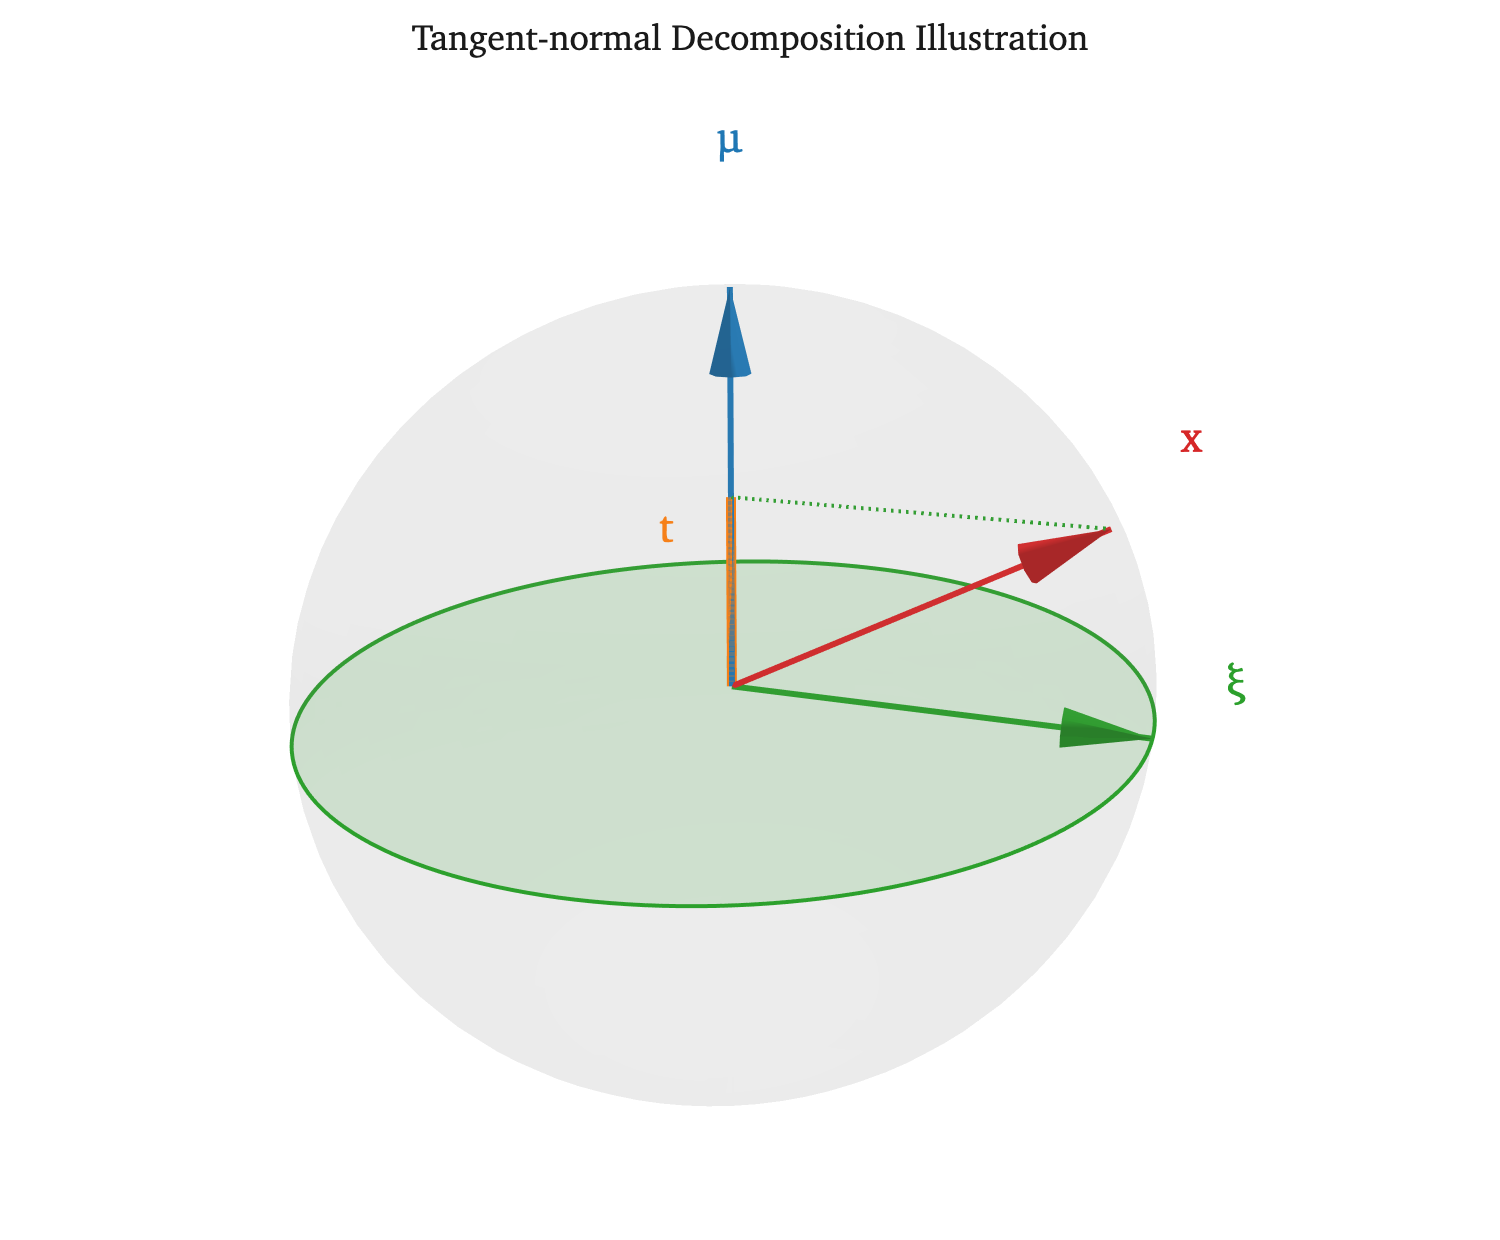
\includegraphics[trim=289 133 254 23, clip, width=\textwidth]{assets/tangent_normal_decomposition.png}
    \label[figure]{fig:tangent-normal-illustration}
\end{minipage}

The statements and intuition that follow are largely introduced in \cite{decao2020powersphericaldistribution} and
\cite{mardia2009directional}.
\begin{theorem}[Marginal density of rotationally-symmetric distributions]
\label{thm:marginal}
Consider the tangent-normal decomposition of a unit vector $\mathbf{x} \in \mathbb{S}^{d - 1}$. The Lebesgue density of
$t = \boldsymbol{\mu}^\top\mathbf{x}$ is given by
\[
    \sigma_t = B\left(\frac{d - 1}{2}, \frac{1}{2}\right)^{-1}\left(1 - t^2\right)^{\frac{d - 3}{2}}
\]
Consequently, if $f(\mathbf{x}; \boldsymbol{\mu}, \boldsymbol{\Theta})$ is a rotationally-symmetric distribution on the
unit hypersphere, it may be written in terms of its \textit{angular density} \citep{Garc_a_Portugu_s_2019} $g\left(\boldsymbol{\mu}^\top\mathbf{x}; \boldsymbol{\Theta}\right)$:
\[
    f(\mathbf{x}; \boldsymbol{\mu}, \boldsymbol{\Theta}) = \frac{g\left(\boldsymbol{\mu}^\top\mathbf{x}; \boldsymbol{\Theta}\right)}{\sigma_t}
\]
Additionally, $g$ may be written as
\[
    g\left(t; \boldsymbol{\Theta}\right) = C_T(\boldsymbol{\Theta})\phi(t; \boldsymbol{\Theta})\sigma_t
\]
where $C_T(\cdot)$ is a normalizing constant.
\end{theorem}
It thus suffices to consider rotationally-symmetric distributions on the unit hypersphere by their respective $\phi(t; \boldsymbol{\Theta})$ as
in \Cref{thm:marginal}. For the sake of brevity, we refer to these identifiers as \textit{angular kernels}.
\begin{example}
The \textit{von Mises-Fisher} (vMF) distribution with mean direction $\boldsymbol{\mu}$ and concentration $\kappa$ is a
rotationally-symmetric distribution with angular kernel $\phi(t; \kappa) = \exp(\kappa t)$. The full density is given by
\[
    f(\mathbf{x}; \boldsymbol{\mu}, \kappa) = \frac{\kappa^{\frac{d}{2} - 1}}{(2\pi)^{\frac{d}{2}}I_{\frac{d}{2} - 1}(\kappa)}\exp\left(\kappa\boldsymbol{\mu}^\top\mathbf{x}\right)
\]
as outlined in \cite{davidson2022hypersphericalvariationalautoencoders}, where $I_v$ denodes the modified Bessel function at
order $v$.
\end{example}
\begin{example}
The \textit{power-spherical} distribution \citep{decao2020powersphericaldistribution} with mean direction $\boldsymbol{\mu}$ and concentration $\kappa$ is a
rotationally-symmetric distribution with angular kernel $\phi(t; \kappa) = (1 + t)^\kappa$. The full density is given by
\[
    f(\mathbf{x}; \boldsymbol{\mu}, \kappa) = \left[ 2^{\alpha + \beta}\pi^\beta \frac{\Gamma(\alpha)}{\Gamma(\alpha + \beta)} \right]^{-1}\left(1 + \boldsymbol{\mu}^\top\mathbf{x}\right)^\kappa, \qquad \alpha = \frac{d - 1}{2} + \kappa, \beta = \frac{d - 1}{2}
\]
Both the vMF and power-spherical distributions can be considered as ``location-scale'' distributions on the unit
hypersphere, almost as spherical analogues to the normal distribution. 
\end{example}
\begin{figure}[H]
    \centering
    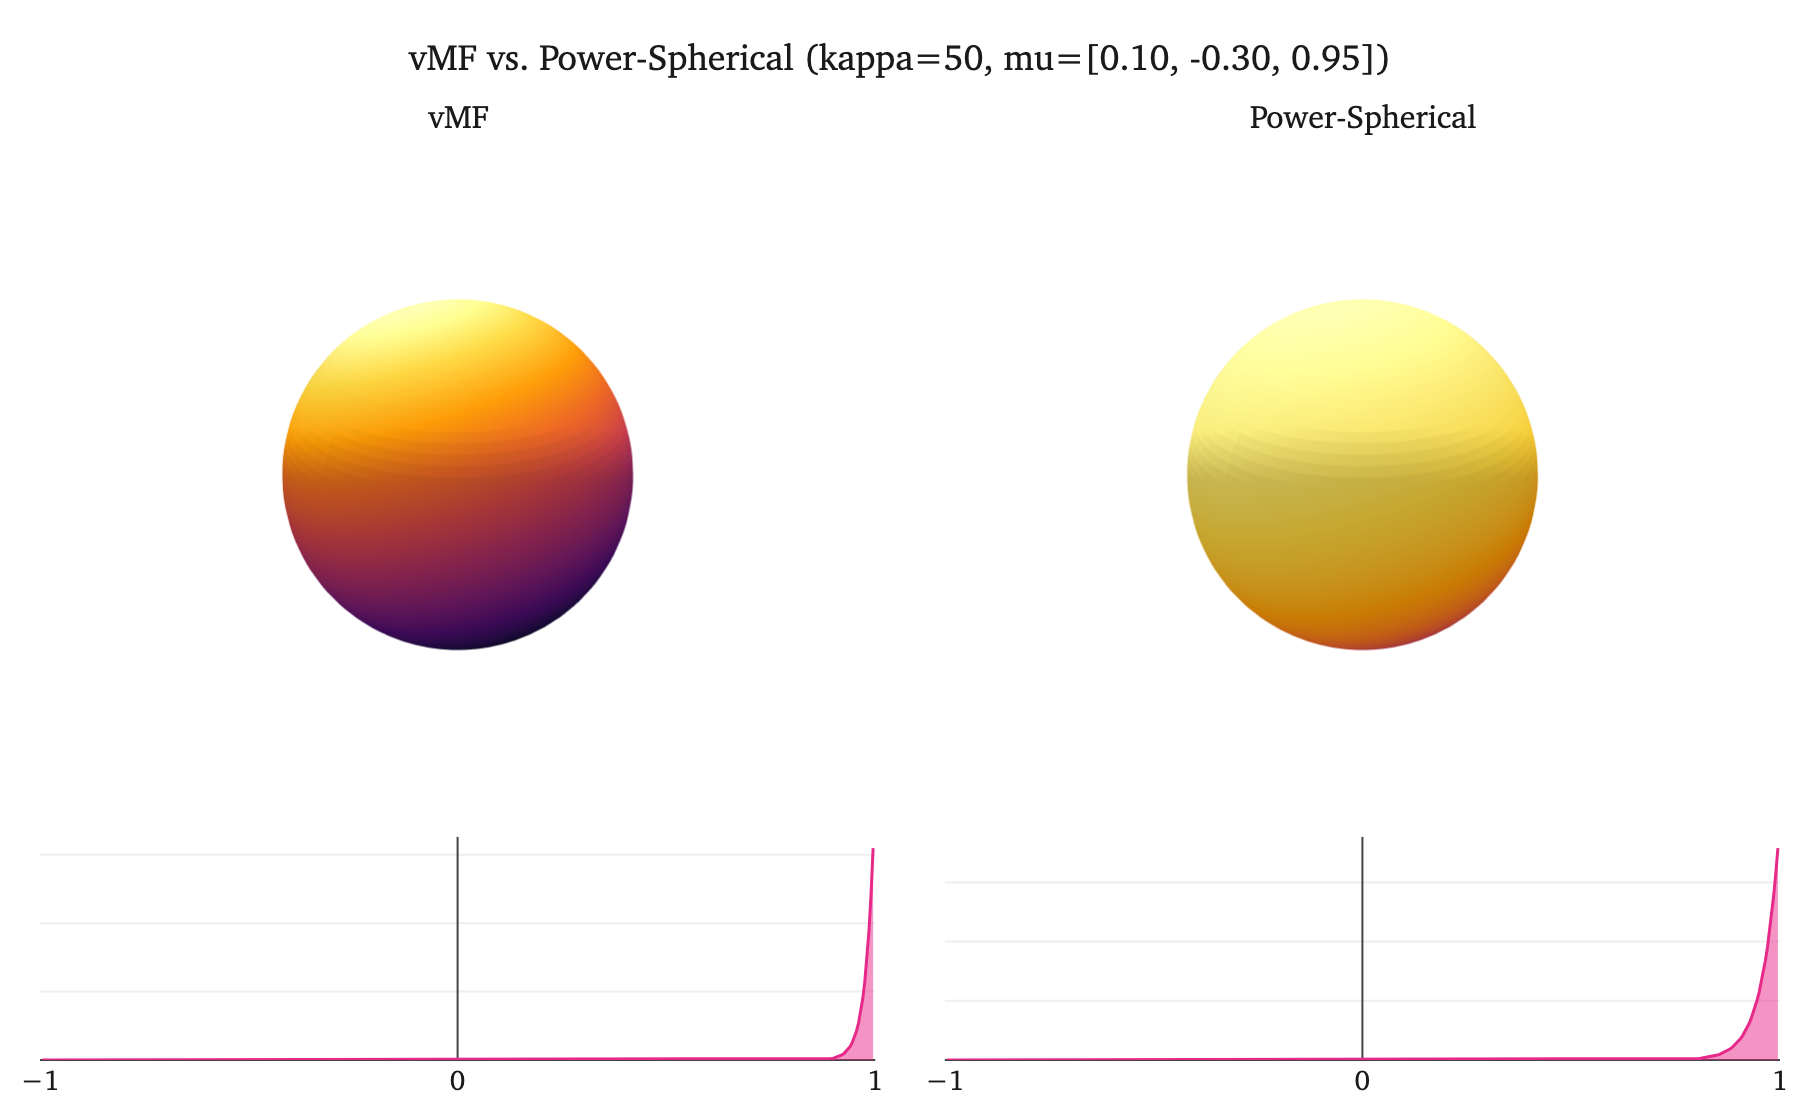
\includegraphics[width=\textwidth]{assets/location_scale_comparison.png}
    \caption{Von Mises-Fisher (left) and power-spherical (right) on $\mathbb{S}^2$ at the same mean direction
    $\boldsymbol{\mu} = (0.1, -0.3, 0.95)$ and the same concentration $\kappa = 50$: a log-density heatmap on the
    sphere above each family's univariate angular density $g(t; \kappa)$ below.}
    \label{fig:vmf-power-spherical-comparison}
\end{figure}
Aside from lighter tails, the power-spherical distribution distinguishes itself from the vMF distribution
through significantly faster sampling and numerically stable density evaluation. Since the vMF distribution's
angular density depends on the modified Bessel function, it does not admit an inverse CDF. As such, producing vMF samples
requires rejection sampling as outlined in \cite{davidson2022hypersphericalvariationalautoencoders}. The power-spherical
distribution, on the other hand, can be produced by a deterministic transformation of a beta-distributed sample:
\[
    X  = 2Z - 1, \qquad Z \sim \text{Beta}\left(\frac{d - 1}{2} + \kappa, \frac{d - 1}{2}\right)
\]
Above, $X$ follows the angular density of a power-spherical distribution. It is important to note, however, that both
of the above distributions are limited in their expressivity:
\begin{theorem}[Modality of the vMF and Power-Spherical Distributions]
\label{thm:locscale-modality}
For any mean direction $\boldsymbol{\mu} \in \mathbb{S}^{d - 1}$ and concentration $\kappa > 0$, the vMF and
power-spherical distributions are unimodal with unique mode at $\boldsymbol{\mu}$.
\end{theorem}
Below, we introduce a new distribution on the unit hypersphere which admits greater expressivity.
